\chapter{Introduzione}\label{cap:introduzione}

\section{Contesto}\label{sez:contesto}

A seguito della crescita esponenziale del web in questo secolo e dell'abituarsi di tutti coloro che ne usufruiscono ad un livello grafico sempre migliore e ad una esperienza mano a mano pi\`u interattiva e vicina all'utente medio, i siti web e le tecnologie utilizzate si sono adattati per permettere uno sviluppo sempre pi\`u rapido di codice pi\`u facilmente testabile e mantenibile.

Di conseguenza nel frontend si sono susseguiti una serie di framework e di strumenti, a partire da JQuery\cite{jquery} nel 2006, che per primo si \`e occupato di risolvere il problema della compatibilit\`a tra browsers, permettendo ai developers di scrivere una volta, e poter eseguire su tutti i browsers.

AngularJS nel 2010 \`e stato il primo MVC framework ad offrire in un unico pacchetto un insieme di features che hanno facilitato molto la vita agli sviluppatori, come il two-way data binding, la dependency injection, il routing integrato, ed altri strumenti utili per rendere pi\`u standard lo sviluppo nel frontend~\cite{Hoff}.
AngularJS pur essendo stato largamente utilizzato, \`e stato cambiato radicalmente nel 2013 e rinominato in Angular2 (e nelle versioni pi\`u recenti semplicemente Angular) senza mantenere retrocompatibilit\`a e senza offrire un modo preciso per migrare alla nuova versione ai precedenti utilizzatori di AngularJS.
Anche per questo motivo, React, un nuovo framework pi\`u leggero e modulare mantenuto da Facebook e la cui prima versione risale proprio al 2013, ha mano a mano preso il posto di Angular come framework pi\`u utilizzato nel frontend.

Vue infine \`e il terzo dei principali framework moderni per la creazione di interfacce utente che \`e stato fortemente adottato, proponendo una versione intermedia tra il pi\`u opinionato Angular e il pi\`u flessibile React, lanciato nel 2014~\cite{vueJs}.

Oltre a questi, ciascuno con la propria semantica, organizzazione logica delle cartelle, spesso una CLI dedicata, ad un developer frontend viene solitamente richiesto di conoscere HTML, CSS e chiaramente Javascript essendo ci\`o su cui si basano poi i vari framework, jQuery per retrocompatibilit\`a e Bootstrap(solitamente sia versione 3 che 4) per creare componenti standard pi\`u in fretta.

Oltre a Javascript, se si vuole scrivere degli unit test facilmente mantenibili, bisogna conoscere TypeScript(specialmente se si utilizza Angular, che rende il suo utilizzo obbligatorio).
TypeScript in particolare \`e un linguaggio di programmazione che estende la sintassi di Javascript, rendendolo tipizzato(e non interpretato), e viene quindi compilato e trasformato in codice equivalente nel linguaggio javascript, per poter essere utilizzato dal browser.
Questo processo di compilazione e traduzione da un linguaggio verso l'altro, prende il nome di transpilazione.

\section{Problema}\label{sez:problema}
I continui cambiamenti nei molti framework utilizzati, la diversit\`a degli strumenti tra loro, che spesso realizzano in modo diverso la stessa cosa, rendono sempre pi\`u difficile per un junior developer iniziare a sviluppare, vista l'ampia curva di apprendimento e quindi il tempo e lo studio necessario, per poter essere pronto a lavorare come un professionista.

Oltretutto un web developer ad oggi finisce per essere costretto a scegliere se diventare uno sviluppatore frontend o backend, dato che rimanere al passo e aggiornarsi gi\`a in solo uno di questi due campi richiede molto tempo ed impegno, spesso oltre l'orario di lavoro.

\`E quindi chiaro che da parte di tutti i web developer, e specialmente per una figura mista spesso identificata con il titolo "Full-Stack Developer", ci sia una continua ricerca del modo per rendere le proprie competenze quanto pi\`u trasversali possibile, anche in termini di tecnologie utilizzate.

\pagebreak

\section{Linguaggi General-Purpose}\label{sez:linguaggiGeneralPurpose}
Microsoft, nel backend e in ambito applicativo, ha reso nel tempo il framework .NET Standard e le sue implementazioni(la piattaforma .NET Core, il .NET Framework e Mono) utilizzabili nei vari linguaggi sviluppati da Microsoft ovvero C\#, F\# e VB.
La figura \ref{fig:DotNetImplementations} di seguito riassume le implementazioni del .NET Standard e le varie tipologie di applicazioni che si possono sviluppare con ciascuna.

\begin{figure}[H]
	\centerline{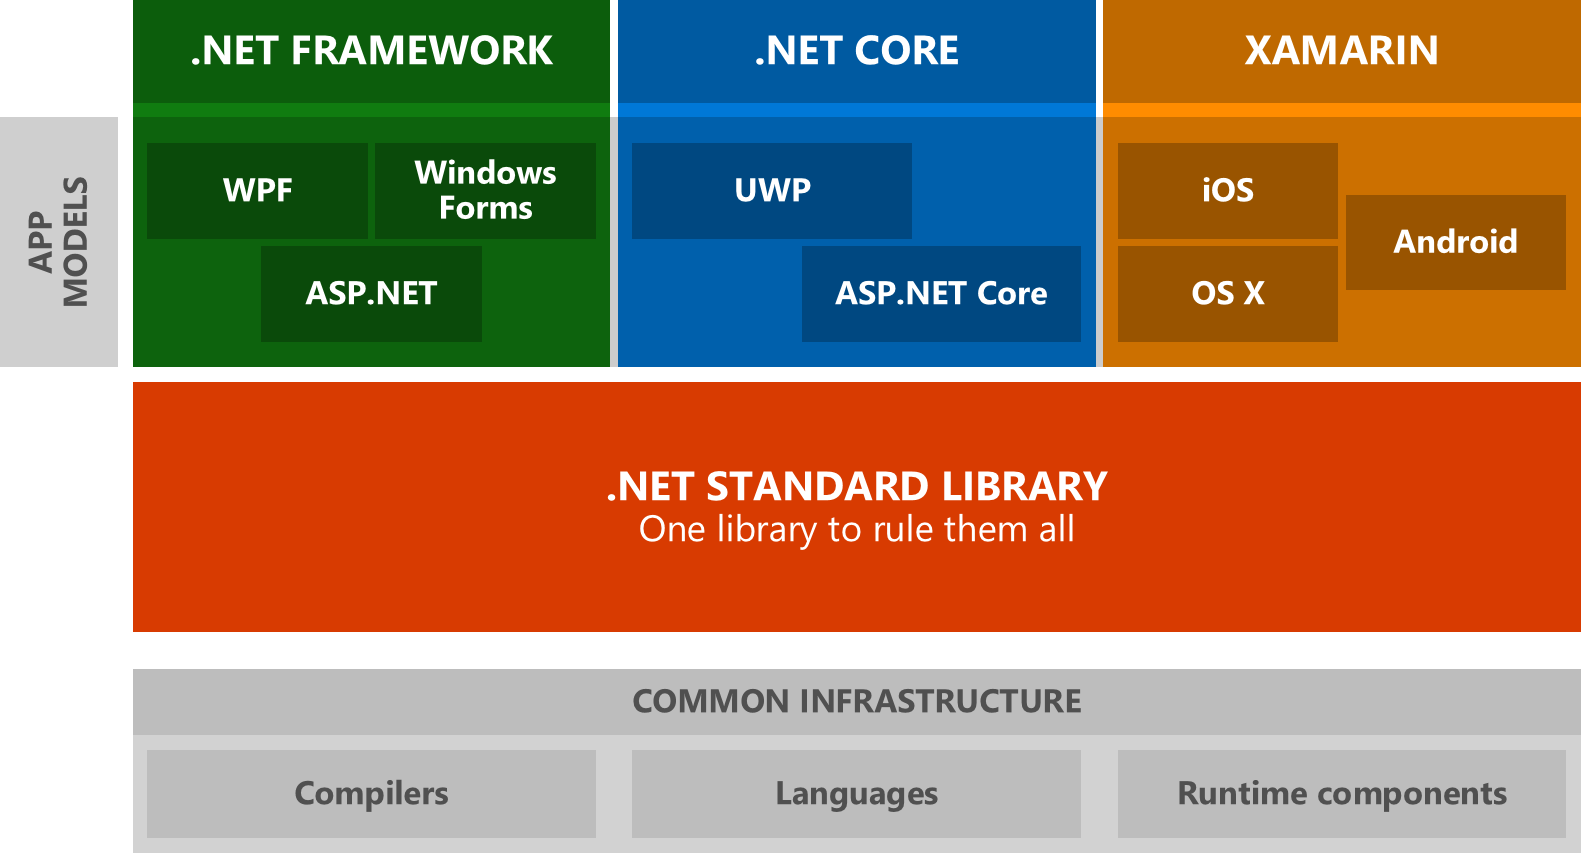
\includegraphics[scale=0.2]{figure/DotNetImplementations}}
	\caption{Implementazioni del .NET Standard}
	\label{fig:DotNetImplementations}
\end{figure}

Scrivendo ad esempio in C\# \`e possibile sviluppare vari tipi di applicazioni come si pu\`o vedere nella figura \ref{fig:DotNetCapabilities}, ma se si decide di sviluppare codice per un'applicazione web che gestisca eventi del Browser(click, drag, hover,...) ad oggi si \`e costretti a scriverla utilizzando Javascript.
Eventualmente sfruttando anche un framework se si vuole essere pi\`u veloci nello sviluppo e scrivere codice mantenibile specialmente se a livello enterprise.

\begin{figure}[H]
\centerline{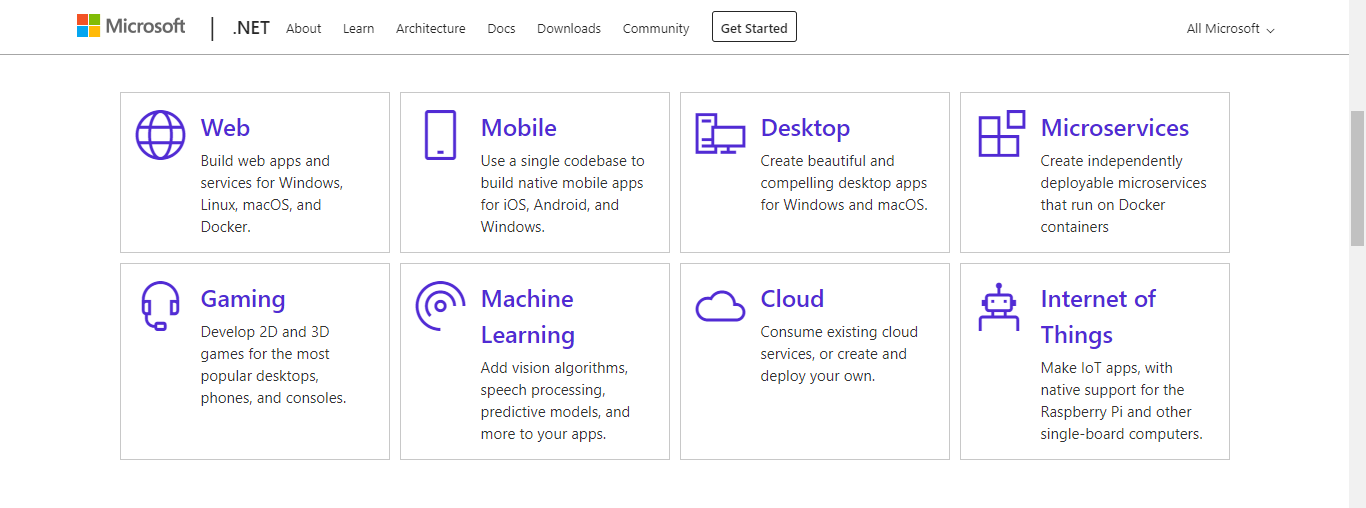
\includegraphics[scale=0.35]{figure/DotNetFrameworkCapabilities}}
\caption{Possibilit\`a di .NET}
\label{fig:DotNetCapabilities}
\end{figure}

Gi\`a con Razor\cite{razor}, Microsoft ha permesso la generazione di codice HTML e CSS in modo dinamico utilizzando C\#, ma questa tecnologia per il server-side rendering \`e utilizzabile solo lato server e quindi la cattura di un evento client side come il click di un utente su un bottone, senza passare per il server sul quale viene eseguito l'hosting dell'applicazione, non \`e stato possibile utilizzando esclusivamente questa tecnologia.

\section{Blazor}
Ecco cosa \`e quindi Blazor: la versione pi\`u avanzata di Razor(Browser+Razor\cite{blazorWikiGitHub}), o meglio ancora un Framework per la creazione di User Interfaces(da qui in poi UI) di Single Page Application(da qui in poi SPA) che permette ai developer di gestire anche gli eventi client-side, direttamente in C\# o nel linguaggio scelto tra quelli supportati.
Questo framework come se il linguaggio scelto fosse effettivamente ci\`o che viene eseguito dal client, mentre in realt\`a ci\`o che viene eseguito lato client cambia a seconda del modello scelto, come poi vedremo pi\`u nel dettaglio.

Blazor utilizza per i vari modelli, delle tecnologie diverse(ad esempio il WebAssembly) ma che rispettano sempre lo standard del web.

Non \`e un plugin da installare, e non dipende da un browser specifico.
Non \`e una tecnologia che sfrutta la transpilazione verso javascript, contrariamente a TypeScript.